\documentclass{pssbmac}

%%%%%%%%%%%%%%%%%%%%%%%%%%%%%%%%%%%%%%%%%%%%%%%%%%%%%%%%%%%%%%%%%%%%%%%%
%% POR FAVOR, NÃO FAÇA MUDANÇAS NESSE PADRÃO QUE ACARRETEM  EM
%% ALTERAÇÃO NA FORMATAÇÃO FINAL DO TEXTO
%%%%%%%%%%%%%%%%%%%%%%%%%%%%%%%%%%%%%%%%%%%%%%%%%%%%%%%%%%%%%%%%%%%%%%%%

%%%%%%%%%%%%%%%%%%%%%%%%%%%%%%%%%%%%%%%%%%%%%%%%%%%%%%%%%%%%%%%%%%%%%%%%
% POR FAVOR, ESCOLHA CONFORME O CASO
%%%%%%%%%%%%%%%%%%%%%%%%%%%%%%%%%%%%%%%%%%%%%%%%%%%%%%%%%%%%%%%%%%%%%%%%
\usepackage[brazil]{babel} % texto em Português
%\usepackage[english]{babel} % texto em Inglês

%\usepackage[latin1]{inputenc} % acentuação em Português ISO-8859-1
\usepackage[utf8]{inputenc} % acentuação em Português UTF-8
%%%%%%%%%%%%%%%%%%%%%%%%%%%%%%%%%%%%%%%%%%%%%%%%%%%%%%%%%%%%%%%%%%%%%%%%


%%%%%%%%%%%%%%%%%%%%%%%%%%%%%%%%%%%%%%%%%%%%%%%%%%%%%%%%%%%%%%%%%%%%%%%%
%% POR FAVOR, NÃO ALTERAR
%%%%%%%%%%%%%%%%%%%%%%%%%%%%%%%%%%%%%%%%%%%%%%%%%%%%%%%%%%%%%%%%%%%%%%%%
\usepackage[T1]{fontenc}
\usepackage{float}
\usepackage{graphics}
\usepackage{graphicx}
\usepackage{epsfig}
\usepackage{indentfirst}
\usepackage{amsmath, amsfonts, amssymb, amsthm, mathtools}
\usepackage{url}
\usepackage{csquotes}
% Ambientes pré-definidos
\newtheorem{theorem}{Theorem}[section]
\newtheorem{lemma}{Lemma}[section]
\newtheorem{proposition}{Proposition}[section]
\newtheorem{definition}{Definition}[section]
\newtheorem{remark}{Remark}[section]
\newtheorem{corollary}{Corollary}[section]
\newtheorem{teorema}{Teorema}[section]
\newtheorem{lema}{Lema}[section]
\newtheorem{prop}{Proposi\c{c}\~ao}[section]
\newtheorem{defi}{Defini\c{c}\~ao}[section]
\newtheorem{obs}{Observa\c{c}\~ao}[section]
\newtheorem{cor}{Corol\'ario}[section]

% ref bibliográficas
\usepackage[backend=biber, style=numeric-comp, maxnames=50]{biblatex}
%adicionados
\usepackage{enumitem}
\usepackage{algorithm}
\usepackage{algorithmic}
\usepackage{mdframed}


\addbibresource{refs.bib}
\DeclareTextFontCommand{\emph}{\boldmath\bfseries}
\DefineBibliographyStrings{brazil}{phdthesis = {Tese de doutorado}}
\DefineBibliographyStrings{brazil}{mathesis = {Disserta\c{c}\~{a}o de mestrado}}
\DefineBibliographyStrings{english}{mathesis = {Master dissertation}}
%%%%%%%%%%%%%%%%%%%%%%%%%%%%%%%%%%%%%%%%%%%%%%%%%%%%%%%%%%%%%%%%%%%%%%%%


\begin{document}

%%%%%%%%%%%%%%%%%%%%%%%%%%%%%%%%%%%%%%%%%%%%%%%%%%%%%%%%%%%%%%%%%%%%%%%%
% TÍTULO E AUTORAS(ES)
%%%%%%%%%%%%%%%%%%%%%%%%%%%%%%%%%%%%%%%%%%%%%%%%%%%%%%%%%%%%%%%%%%%%%%%%

\title{Otimização Multiobjetivo para Planejamento de Rotas Turísticas: Um Dia no Rio de Janeiro}

\author{
    {\large Augusto Magalhães Pinto de Mendonça}\thanks{augustompm@id.uff.br}\\
    {\small IC/UFF, Niteroi, RJ} \\
    {\large Filipe Pessôa Sousa}\thanks{filipe.sousa@pos.ime.uerj.br}\\
    {\small IME/UERJ, Rio de Janeiro, RJ} \\    
    {\large Igor Machado Coelho}\thanks{imcoelho@ic.uff.br}\\
    {\small IC/UFF, Niteroi, RJ} \\
}
\criartitulo
%%%%%%%%%%%%%%%%%%%%%%%%%%%%%%%%%%%%%%%%%%%%%%%%%%%%%%%%%%%%%%%%%%%%%%%%


%%%%%%%%%%%%%%%%%%%%%%%%%%%%%%%%%%%%%%%%%%%%%%%%%%%%%%%%%%%%%%%%%%%%%%%%
% TEXTO
%%%%%%%%%%%%%%%%%%%%%%%%%%%%%%%%%%%%%%%%%%%%%%%%%%%%%%%%%%%%%%%%%%%%%%%%

\begin{abstract}
{\bf Resumo}. Este trabalho apresenta uma abordagem de otimização multiobjetivo para o planejamento de rotas turísticas de um dia no Rio de Janeiro. O problema foi modelado com quatro objetivos: Minimização dos custos e do tempo de deslocamento, e maximização das atrações visitadas e da diversidade de bairros.
%minimização de custos, minimização de tempo de deslocamento, maximização de atrações visitadas e maximização da diversidade de bairros
Este trabalho apresenta uma abordagem de otimização multiobjetivo para o planejamento de rotas turísticas de um dia no Rio de Janeiro. O problema foi modelado com quatro objetivos: Minimização dos custos e do tempo de deslocamento, e maximização das atrações visitadas e da diversidade de bairros. 

\noindent
{\bf Palavras-chave}. Otimização Combinatória, Otimização Multiobjetivo, Metaheurística, NSGA-II, Roteirização Turística.
\end{abstract}

\section{Introdução}

O planejamento de rotas turísticas apresenta desafios de otimização, especialmente quando múltiplos critérios conflitantes precisam ser considerados simultaneamente. Ao estruturar um roteiro que busque minimizar custos e tempos de deslocamento enquanto maximiza o número de atrações visitadas e a diversidade de bairros, observamos objetivos naturalmente conflitantes que exigem técnicas especializadas para sua resolução. Estas características tornam tal problema adequado para abordagens de otimização multiobjetivo, possibilitando que turistas possam explorar eficientemente os pontos turísticos sem comprometer a qualidade da experiência, respeitando restrições práticas como horários de funcionamento, orçamentos disponíveis e limitações de distância.

Os algoritmos evolutivos multiobjetivo surgiram formalmente em 1985 com o VEGA de Schaffer~\cite{Schaffer1985}, que revolucionou a abordagem para problemas com objetivos conflitantes. No entanto, foi o NSGA-II desenvolvido por Deb et al. em 2002~\cite{Deb2002}  que trouxe avanços decisivos ao superar limitações críticas: reduziu a complexidade computacional de O(MN³) para O(MN²), implementou elitismo ao combinar populações pai e descendente, e eliminou a necessidade de parâmetros de compartilhamento através de um operador de comparação populacional que preserva a diversidade.


O planejamento de rotas turísticas no Rio de Janeiro representa um desafio particular devido à diversidade de atrações distribuídas pela cidade, muitas das quais permanecem pouco exploradas mesmo pelos moradores locais. Como Machado \cite{Machado2013} observa em seu estudo sobre a evolução do turismo na cidade, o Rio possui uma longa tradição de visitação que remonta ao período imperial, tendo atraído admiração por sua paisagem desde o século XIX, embora inicialmente carecesse de infraestrutura adequada. Atualmente, o problema envolve não apenas identificar pontos turísticos relevantes, mas otimizar roteiros considerando as limitações de tempo e orçamento dos visitantes. 

Para viabilizar a modelagem do problema de roteirização turística, foram utilizadas duas principais fontes de dados. O TripAdvisor \cite{TripAdvisor2024}, plataforma colaborativa que agrega avaliações e informações sobre destinos turísticos, forneceu dados estruturados sobre as atrações cariocas. A partir do ranking de popularidade e qualidade da plataforma, foram selecionadas as 40 atrações mais bem classificadas do Rio de Janeiro, extraindo-se informações de custos, tempos médios de visitação e horários de funcionamento. Para as informações de deslocamento entre atrações, o estudo utilizou dados do OpenStreetMap \cite{OpenStreetMap2024}, projeto colaborativo de mapeamento global com licença aberta. Por meio do Open Source Routing Machine (OSRM) e do serviço derivado Mapbox \cite{Mapbox2024}, foram obtidas as matrizes de tempo e distância para deslocamentos de carro e a pé entre todas as atrações mapeadas. A formulação dos custos de transporte baseou-se em uma análise dos preços praticados por empresas de transporte por aplicativo na cidade, chegando-se ao valor médio de R\$6,00 por quilômetro percorrido. 

Com base nessas fontes de dados, nosso estudo se propõe a três objetivos fundamentais: implementar e avaliar o algoritmo NSGA-II para resolver o problema de roteirização turística multiobjetivo; quantificar a qualidade das soluções geradas através da métrica de hipervolume; e disponibilizar um aplicativo web de código aberto desenvolvido com Flask \cite{Flask2024} e Dash \cite{Dash2024} que permita aos usuários navegar intuitivamente entre as diversas soluções otimizadas.

O restante deste trabalho está organizado da seguinte forma: a Seção 2 apresenta a fundamentação teórica sobre problemas de otimização multiobjetivo; a Seção 3 detalha a metodologia adotada, incluindo a modelagem do problema com suas funções objetivo e restrições; a Seção 4 expõe os resultados obtidos com imagens do protótipo de aplicativo desenvolvido; e, por fim, a Seção 5 apresenta as conclusões e sugere direções para trabalhos futuros.


\section{Referencial Teórico}

Algoritmos genéticos, formalizados por Holland \cite{Holland1973}, representam técnicas de otimização inspiradas na evolução biológica que abordam problemas complexos através de populações de soluções que evoluem por seleção, cruzamento e mutação. Esta analogia com processos naturais tem sido aplicada no contexto turístico, como demonstrado por Choi et al. \cite{Choi2022}, que utilizaram estas técnicas para otimizar o tempo total dos itinerários. Contudo, o problema de roteirização turística mostra-se complexo,  propício para o uso de algoritmos multiobjetivos, que buscam equilibrar diferentes critérios.

A área de otimização multiobjetivo evoluiu significativamente desde o trabalho de Schaffer \cite{Schaffer1985}, que desenvolveu o Vector Evaluated Genetic Algorithm (VEGA), dividindo a população em subgrupos orientados a objetivos específicos, até estudos de Zitzler, Deb e Thiele \cite{zitzler2000comparison}, que identificou características específicas influenciando o desempenho algorítmico e evidenciou que nenhuma abordagem dominava completamente as demais em todos os cenários, ressaltando a importância de escolher algoritmos adequados para cada contexto específico. De particular relevância para nossa pesquisa, Arbolino et al. \cite{Arbolino2021} utilizaram otimização multiobjetivo no planejamento sustentável do turismo, equilibrando fatores ambientais, sociais e econômicos na seleção de projetos turísticos, comprovando a superioridade desta técnica na alocação de recursos quando comparada às abordagens tradicionais.

O NSGA-II, desenvolvido por Deb e colaboradores \cite{Deb2002}, consolidou-se como referência em otimização multiobjetivo ao superar limitações críticas de versões anteriores: reduziu a complexidade computacional de $O(MN^3)$ para $O(MN^2)$, implementou um operador de comparação de aglomeração que preserva a diversidade populacional sem parâmetros adicionais, e adotou uma estratégia elitista que incorpora os melhores indivíduos das populações pai e descendente. Seu desempenho competitivo em convergência e manutenção da diversidade de soluções, aliado à eficiência computacional, justifica sua ampla adoção em problemas práticos e sua adequação particular para o problema de roteirização turística abordado neste trabalho.

A avaliação de algoritmos de otimização multiobjetivo apresenta desafios significativos, como demonstrado por Zitzler et al. \cite{Zitzler2003}, que identificaram a insuficiência de indicadores unários e a necessidade de métricas binárias para capturar relações de dominância entre soluções. O hipervolume destaca-se como métrica Pareto-conforme, apesar de sua complexidade exponencial tradicional, limitação enfrentada pelo algoritmo HSO (\textit{Hypervolume by Slicing Objectives}) de While et al. \cite{While2006}, que alcança eficiência superior através do processamento sequencial de objetivos, e complementado por Wang et al. \cite{Wang2023} com técnicas de normalização adaptativa. Em nosso trabalho, implementamos ambas as abordagens para avaliar a qualidade das soluções e aprimorar o processo de busca do NSGA-II, garantindo cobertura mais uniforme da fronteira de Pareto para o problema de roteirização turística.

\section{Metodologia}
O problema de planejamento de rotas turísticas é formulado como um problema de otimização combinatória multiobjetivo. Uma solução consiste em um roteiro de visitas às atrações turísticas, definindo a sequência de visitas, os modos de transporte entre elas e os horários de chegada e partida em cada atração.do Rio de Janeiro.

O modelo tem quatro funções objetivo (Equações \ref{eq:custo}-\ref{eq:bairros}): minimizar custo (\(Z_1\)), tempo (\(Z_2\)), e maximizar atrações (\(Z_3\)) e bairros distintos visitados (\(Z_4\)):
\begin{align}
Z_1 &= \sum_{i,j \in A} x_{ij}(e_i + c_{ij}(m_{ij})) &&\text{(Custo total)} \label{eq:custo}\\[3pt]
Z_2 &= \sum_{i,j \in A} x_{ij}(t_{ij}(m_{ij}) + v_i) + \sum_{i \in A} w_i &&\text{(Tempo total)} \label{eq:tempo}\\[3pt]
Z_3 &= -\sum_{i \in A}\min(1, \sum_{j \in A} x_{ij}) &&\text{(Qtd. atrações)} \label{eq:atracoes}\\[3pt]
Z_4 &= -|\{b_i | i \in A, \sum_{j \in A} x_{ij} \geq 1\}| &&\text{(Diversidade bairros)} \label{eq:bairros}
\end{align}
{\small Onde \(c_{ij}(m_{ij})=0\) se caminhada e R\$6/km se carro.}
\\
\\
As principais variáveis e parâmetros do modelo são:
\begin{description}[noitemsep,topsep=0pt,parsep=0pt,leftmargin=!,labelwidth=\widthof{\bfseries \(m_{ij}\)}]
    \item[\(t_{ij}^{\text{walk}}\)] Tempo de deslocamento a pé entre atrações \( i \) e \( j \).
    \item[\(d_{ij}\)] Distância em metros entre atrações \( i \) e \( j \).
    \item[\(0, n\)] Índices especiais representando ponto de partida e chegada do roteiro.
    \item[\(k\)] Índice das atrações intermediárias (exclui o ponto de partida \(0\) e o destino final \(n\)).
    \item[\(x_{ij}\)] Variável binária indicando se o turista vai da atração \( i \) para a \( j \) (1 sim, 0 não).
    \item[\(m_{ij}\)] Variável binária para modo de transporte entre \( i \) e \( j \): caminhada (0) ou carro (1).
    \item[\(a_i\)] Horário de chegada na atração \( i \).
    \item[\(d_i\)] Horário de partida da atração \( i \).
    \item[\(t_{ij}\)] Tempo de deslocamento entre \( i \) e \( j \) com transporte escolhido.
    \item[\(c_{ij}\)] Custo do deslocamento entre \( i \) e \( j \) com transporte escolhido.
    \item[\(v_i\)] Tempo de visitação da atração \( i \).
    \item[\(w_i\)] Tempo de espera na atração \( i \) quando chegada ocorre antes da abertura.
    \item[\(e_i\)] Custo de entrada na atração \( i \).
    \item[\(b_i\)] Bairro onde está localizada a atração \( i \).
    \item[\(O_i\)] Horário de abertura da atração \( i \).
    \item[\(F_i\)] Horário de fechamento da atração \( i \).
\end{description}
\vspace{1em}
O modelo é sujeito às oito restrições a seguir (Equações 5-11), apresentadas na Tabela 1:
\begin{table}[ht]
\scriptsize
\caption{Conjunto de restrições do modelo de roteirização turística (Equações 5-11).}
\label{tab:constraints}
\begin{flushleft}
\begin{tabular}{@{}rl@{}}
\toprule
(5) &
$\displaystyle
\sum_{i,j \in A} x_{ij}\bigl(t_{ij}(m_{ij}) + v_i\bigr) + \sum_{i\in A} w_i \;\leq\; 840 
\quad\text{(Tempo diário)}$
\\[3pt]
(6) &
$\displaystyle
O_i \;\leq\; a_i \;\leq\; d_i \;\leq\; F_i,\quad 
d_i - a_i \;\geq\; v_i 
\quad \forall i \in A:\; \sum_{j \in A} x_{ij} \;\geq\; 1 
\quad\text{(Funcionamento)}$
\\[3pt]
(7) &
$\displaystyle
a_j \;\geq\; d_i + t_{ij}(m_{ij})
\quad \forall i,j \in A:\; x_{ij}=1
\quad\text{(Sequencialidade)}$
\\[3pt]
(8) &
$\displaystyle
\sum_{j \in A} x_{ij} \;\leq\; 1, 
\quad
\sum_{i \in A} x_{ij} \;\leq\; 1
\quad \forall i,j \in A
\quad\text{(Unicidade)}$
\\[3pt]
(9) &
$\displaystyle
m_{ij} \;=\;
\begin{cases}
0, & t_{ij}^{\text{walk}}\;\leq\; 15,\\
1, & \text{caso contrário},
\end{cases}
\quad \forall i,j \in A:\; x_{ij}=1
\quad\text{(Preferência transporte)}$
\\[5pt]
(10) &
$\displaystyle
c_{ij}(m_{ij}) \;=\;
\begin{cases}
0, & m_{ij}=0,\\
6 \cdot \dfrac{d_{ij}}{1000}, & m_{ij}=1,
\end{cases}
\quad \forall i,j \in A:\; x_{ij}=1
\quad\text{(Custo carro)}$
\\[5pt]
(11) &
$\displaystyle
\sum_{i \in A} x_{i0}=1,\quad 
\sum_{j \in A} x_{nj}=1,\quad 
\sum_{i \in A} x_{ik}=\sum_{j \in A} x_{kj}
\quad \forall k \in A\setminus\{0,n\}
\quad\text{(Continuidade)}$
\\
\bottomrule
\end{tabular}
\end{flushleft}
\end{table}




\subsection{NSGA-II}
Nossa implementação do Algoritmo~\ref{alg:nsga2} utiliza: (i) seleção por torneio com operador de comparação por dominância e aglomeração (linhas 6-7); (ii) cruzamento específico para sequências de atrações (linha 7); (iii) mutação que adiciona/remove/reordena atrações (linha 7); (iv) mecanismo de penalização para rotas inviáveis durante a avaliação (linha 2). O algoritmo evolui ao longo de $G$ gerações (linha 5), combinando populações pai e descendente (linha 8) e aplicando ordenação não-dominada rápida (linha 9) para produzir um conjunto diverso de roteiros turísticos Pareto-ótimos (linha 17).

\begin{algorithm}[ht!]
\footnotesize 
\caption{Algoritmo NSGA-II adaptado para roteirização turística}
\label{alg:nsga2}
\begin{algorithmic}[1]
\STATE Inicializar população $P_0$ de tamanho $N$
\STATE Avaliar objetivos (custo, tempo, atrações, bairros)
\STATE Classificar $P_0$ por não-dominância: $F = (F_1, F_2, ...)$
\STATE Calcular distância de aglomeração em cada $F_i$
\FOR{$t = 0$ até $G-1$}
  \STATE Selecionar pais de $P_t$ via torneio binário
  \STATE Gerar $Q_t$ (tamanho $N$) via cruzamento e mutação
  \STATE $R_t = P_t \cup Q_t$ (tamanho $2N$)
  \STATE $F = (F_1, F_2, ...)$ = Ordenação-Não-Dominada($R_t$)
  \STATE $P_{t+1} = \emptyset$ e $i = 1$
  \WHILE{$|P_{t+1}| + |F_i| \leq N$}
    \STATE Calcular distância de aglomeração em $F_i$
    \STATE $P_{t+1} = P_{t+1} \cup F_i$ e $i = i + 1$
  \ENDWHILE
  \STATE Ordenar $F_i$ por distância de aglomeração decrescente
  \STATE Incluir primeiros $(N-|P_{t+1}|)$ elementos de $F_i$ em $P_{t+1}$
\ENDFOR
\RETURN Soluções não-dominadas de $P_G$
\end{algorithmic}
\end{algorithm}

\section{Resultados}

Os experimentos foram realizados utilizando dados reais de 40 atrações turísticas do Rio de Janeiro, selecionadas com base no ranking do \textit{TripAdvisor} \cite{TripAdvisor2024}. Esta base inclui pontos turísticos distribuídos por 22 bairros, com tempos de visitação entre 60 e 240 minutos e custos variando de gratuitos a R\$ 844,37. As matrizes de distância e tempo foram construídas utilizando o \textit{Open Source Routing Machine} (OSRM) \cite{OpenStreetMap2024} e o serviço \textit{Mapbox} \cite{Mapbox2024}, fornecendo dados precisos para deslocamentos a pé e de carro. O custo de transporte foi estimado em R\$ 6,00 por quilômetro, baseado nos valores praticados por serviços de transporte por aplicativo na cidade.

Os experimentos foram executados em um processador Intel i7-11700K com 16GB de RAM no sistema operacional Ubuntu 22.04 LTS. O algoritmo NSGA-II foi implementado em C++17. O tempo de execução de cada experimento individual foi de menos de 5 segundos. 

Após testes iniciais, o algoritmo NSGA-II foi configurado com população de 100 indivíduos evoluindo por 100 gerações, utilizando taxa de cruzamento de 0,9 e taxa de mutação de 0,1. Realizamos 30 execuções independentes para garantir robustez estatística dos resultados. Os valores apresentados a seguir representam as médias obtidas nestas execuções.

Em média a execução do NSGA-II resultou em conjuntos de cerca de $70$ soluções não-dominadas, representando roteiros turísticos otimizados com diferentes compensações entre os objetivos. A qualidade das soluções foi avaliada através da métrica de hipervolume, implementada conforme o algoritmo HSO (\textit{Hypervolume by Slicing Objectives}) \cite{While2006}. O conjunto final de soluções alcançou um hipervolume normalizado médio de $0,163$, após aplicação de técnicas de normalização adaptativa conforme proposto por Wang et al. \cite{Wang2023}.

As soluções obtidas apresentam uma ampla gama de resultados: desde roteiros econômicos com média de R\$ 230,21 visitando 8 atrações em 7 bairros em 840 minutos, até roteiros mais dispendiosos com média de R\$ 512,24 que incluem 9 atrações em 8 bairros no mesmo limite de tempo diário. A diversidade de soluções geradas pelo NSGA-II permite aos turistas escolherem roteiros alinhados com suas preferências específicas, equilibrando os quatro objetivos considerados conforme suas prioridades individuais, como pode ser observado na Figura \ref{fig:coordenadas_paralelas}, que ilustra a visualização de coordenadas paralelas das soluções não-dominadas.

\begin{figure}[!ht]
\centering
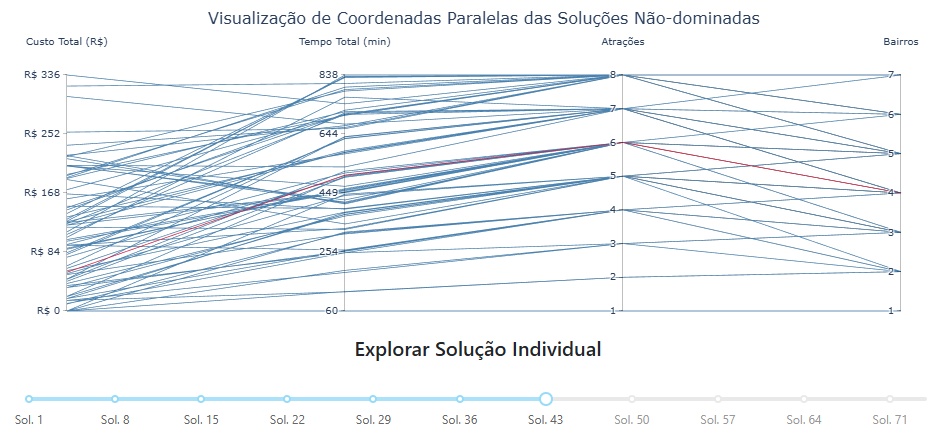
\includegraphics[width=0.80\textwidth]{app1.png}
\caption{Visualização de coordenadas paralelas das soluções não-dominadas. Fonte: Os autores.}
\label{fig:coordenadas_paralelas}
\end{figure}

Para facilitar a exploração das soluções geradas, desenvolvemos um protótipo de aplicativo web denominado "Um Dia no Rio", que permite ao usuário visualizar detalhadamente cada roteiro otimizado, como exemplificado nas Figuras \ref{fig:itinerario} e \ref{fig:linked_arcs}.

\begin{figure}[!ht]
\begin{minipage}[b]{0.40\textwidth}
\centering
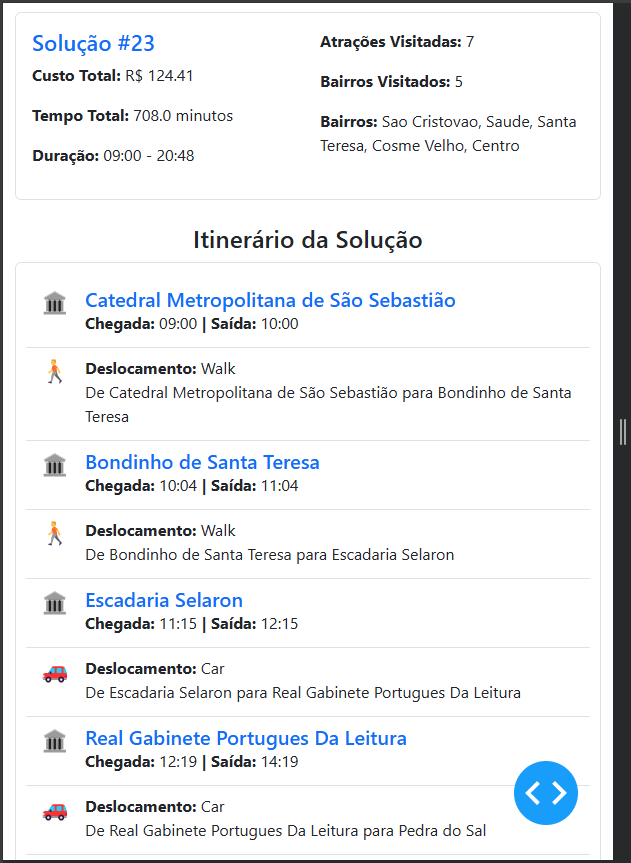
\includegraphics[width=\textwidth]{app2.png}
\caption{Interface do aplicativo "Um Dia no Rio" apresentando um itinerário otimizado. Fonte: Os autores.}
\label{fig:itinerario}
\end{minipage}
\hfill
\begin{minipage}[b]{0.50\textwidth}
\centering
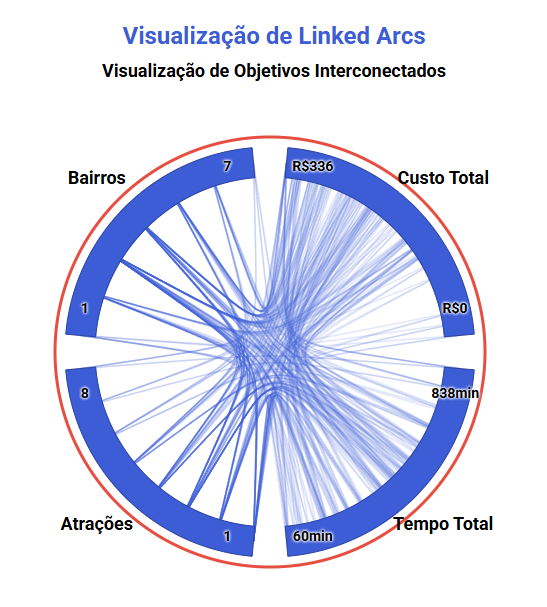
\includegraphics[width=\textwidth]{app3.png}
\caption{Visualização de arcos vinculados entre os objetivos, adaptado de \cite{RoozbehH2023}. Fonte: Os autores.}
\label{fig:linked_arcs}
\end{minipage}
\end{figure}

\section{Conclusão}

Este trabalho apresentou uma abordagem de otimização multiobjetivo para o planejamento de rotas turísticas no Rio de Janeiro utilizando o algoritmo NSGA-II. Os três objetivos propostos foram alcançados: implementamos e avaliamos o NSGA-II para roteirização turística multiobjetivo, adaptando os operadores genéticos para o contexto de sequenciamento de atrações; quantificamos a qualidade das soluções através da métrica de hipervolume; e desenvolvemos o aplicativo web "Um Dia no Rio" que permite aos usuários navegarem entre as soluções otimizadas.

O método proposto mostrou-se capaz de gerar roteiros turísticos de um dia que equilibram quatro objetivos conflitantes: minimização dos custos e do tempo de deslocamento, e maximização das atrações visitadas e da diversidade de bairros
%minimização de custos, minimização de tempo de deslocamento, maximização de atrações visitadas e maximização da diversidade de bairros
, respeitando às restrições práticas essenciais. Os resultados experimentais demonstraram a existência de diversas soluções não-dominadas, oferecendo ao turista opções que variam desde roteiros econômicos até itinerários que maximizam a quantidade e variedade de locais visitados.

Todo o código-fonte desenvolvido neste trabalho está disponível publicamente no repositório GitHub \texttt{https://github.com/augustompm/OM-de-Rotas-Turisticas-Um-Dia-no-Rio}, incluindo a implementação do algoritmo NSGA-II, as estruturas de dados para representação do problema, as ferramentas de análise de hipervolume e o aplicativo web interativo. O arquivo \texttt{README.md} contém instruções detalhadas para execução tanto do aplicativo web (pasta \texttt{app/}) quanto do algoritmo de otimização.

Como trabalhos futuros, identificamos diversas direções promissoras como explorar metodologias alternativas de otimização multiobjetivo, como MOEA/D ou SPEA2, e comparar seu desempenho com o NSGA-II ou incorporar objetivos adicionais, como a preferência pessoal do turista por tipos específicos de atrações.


%%%%%%%%%%%%%%%%%%%%%%%%%%%%%%%%%%%%%%%%%%%%%%%%%%%%%%%%%%%%%%%%%%%%%%%%
% REFS BIBLIOGRÁFICAS
% POR FAVOR, NÃO ALTERAR
%%%%%%%%%%%%%%%%%%%%%%%%%%%%%%%%%%%%%%%%%%%%%%%%%%%%%%%%%%%%%%%%%%%%%%%%
\printbibliography
%%%%%%%%%%%%%%%%%%%%%%%%%%%%%%%%%%%%%%%%%%%%%%%%%%%%%%%%%%%%%%%%%%%%%%%%

\end{document}




